\documentclass[aspectratio=169]{beamer}
\usetheme{Copenhagen}
\usecolortheme{seahorse}
\usepackage{hyperref}
\usepackage{listings}
\usepackage{capt-of}
\usepackage[font=scriptsize]{caption}
\usepackage{pgf}  
\usepackage{booktabs}
\usepackage{epigraph}
\usepackage{tikz}
\usetikzlibrary{calc}
\usetikzlibrary{positioning}
\usetikzlibrary{snakes}
\usepackage{xcolor}
\usepackage{environ}
 
\definecolor{gray}{RGB}{128, 128, 128}
\definecolor{lightgray}{RGB}{200, 200, 200}
\definecolor{cyan}{RGB}{0, 255, 255}
\definecolor{blue}{RGB}{0, 0, 255}
\definecolor{red}{RGB}{255, 0, 0}
\definecolor{pink}{RGB}{255, 128, 128}
\definecolor{green}{RGB}{0, 128, 0}
\definecolor{lightyellow}{RGB}{255, 255, 200}

\lstdefinestyle{all}
    {basicstyle=\ttfamily\scriptsize,
     keywordstyle=\color{blue}\ttfamily\scriptsize,
     commentstyle=\color{green}\ttfamily\scriptsize,
     stringstyle=\color{red}\ttfamily\scriptsize}

\lstset{%
    frame=none,
    xleftmargin=2pt,
    belowcaptionskip=\bigskipamount,
    captionpos=b,
    language=haskell,
    tabsize=2,
    emphstyle={\bf},
    commentstyle=\it,
    morecomment=[l]{--}
    stringstyle=\mdseries\rmfamily,
    alsoletter={},
    keywords={},
    keywords=[1]{instance, case, of, deriving, data, newtype, type, class, if, then, else, where, let, in, do},
    keywords=[2]{MonadTrans, MonadWriter, Num, MonadError, MonadDelay, MonadRace, Semigroup, Monoid, Time, DeltaQ, Show, Read, Eq, Ord, Fractional, Monad, Real, Prob, MonadProb, Functor, Applicative, MonadRandom},
    keywords=[3]{WriterT, ExceptT, Sum, Maybe, RaceS, DelayT, RaceL, Rational, Prize, Strategy, Either, NonEmpty, Double, Bool, Int, ProbS, ProbL, IO, Map},
    keywords=[4]{=>},
    keywords=[5]{Just, Nothing, RS, DT, True, False, DM, RL, Left, Right, Goat, Car, Stay, Change, PS, PL},
    keywordstyle=[1]\bfseries\sffamily\color{red},
    keywordstyle=[2]\bfseries\sffamily\color{blue},
    keywordstyle=[3]\bfseries\sffamily\color{green},
    keywordstyle=[4]\bfseries\sffamily,
    keywordstyle=[5]\bfseries\sffamily\color{black},
    columns=flexible,
    basicstyle=\small\sffamily,
    showstringspaces=false,
    breaklines=false,
    showspaces=false,
}

\title{This ain't your Daddy's Probability Monad}
\subtitle{Haskell eXchange London}
\date{October 10, 2019}
\author{Lars Br\"unjes}
\institute{\includegraphics[width=60mm]{images/IOHK.png}}

\begin{document}

\maketitle

\begin{frame}{Motivation}
    \begin{itemize}
        \item
            Traditional \alert{probability monads}
            are great at modelling uncertainty.
        \item
            Things become more complicated when \alert{time} enters the picture,
            especially in the presence of \alert{concurrency}.
        \item
            Uncertainty, time and concurrency all need to be considered when
            trying to model the behavior of \alert{distributed systems}.
    \end{itemize}
\end{frame}

\begin{frame}{Example: The ``Diamond''-Network}
    \begin{minipage}{0.7\textwidth}%
        \begin{itemize}
            \item
                We consider a network of four nodes, 
                connected as indicated in the diagram.
            \item
                Each individual connection takes a time uniformly distributed
                between one second and two seconds
                and fails with a probability of 10\%.
            \item
                What is the probability for a signal originating in node 1
                to reach node 4? How long will it take?
            \item<2>
                How do time and probability change when an extra edge is added?
        \end{itemize}
    \end{minipage}%
    \begin{minipage}{0.3\textwidth}%
        \centering

        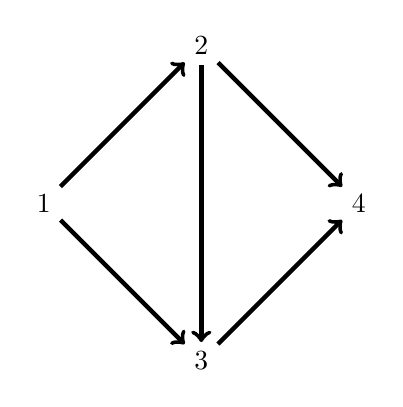
\begin{tikzpicture}[scale=2]
            \node (A) at  (0, 0) {1};
            \node (B) at  (1, 1) {2};
            \node (C) at  (1,-1) {3};
            \node (D) at  (2, 0) {4};
            \draw [ultra thick, ->] (A) -- (B);
            \draw [ultra thick, ->] (A) -- (C);
            \draw<2>[ultra thick, ->] (B) -- (C);
            \draw [ultra thick, ->] (B) -- (D);
            \draw [ultra thick, ->] (C) -- (D);
        \end{tikzpicture}
    \end{minipage}%
\end{frame}

\begin{frame}{Modelling Uncertainty --- {\tt MonadProb}}
    \vspace{-5mm} 
    \lstinputlisting[basicstyle=\scriptsize, firstline=8, lastline=8]
        {code/src/Data/Prob.hs}
    \lstinputlisting[basicstyle=\scriptsize, firstline=10, lastline=11]
        {code/src/Data/Prob.hs}
    \pause
    \lstinputlisting[basicstyle=\scriptsize, firstline=14, lastline=25, backgroundcolor=\color{lightyellow}]
        {code/src/Control/Monad/Probability/Class.hs}
    \lstinputlisting[basicstyle=\scriptsize, firstline=27, lastline=28]
        {code/src/Control/Monad/Probability/Class.hs}
\end{frame}

\begin{frame}{Example: Throwing Dice}
    \begin{minipage}{0.5\textwidth}%
        \lstinputlisting[firstline=12, lastline=18]
            {code/src/Examples/Dice.hs}
    \end{minipage}%
    \begin{minipage}{0.5\textwidth}%
        \centering
        \includegraphics[width=50mm]{images/dice.jpg}
    \end{minipage}
\end{frame}

\begin{frame}{Example: Monty Hall}
    \begin{minipage}[t]{0.75\textwidth}%
        \vspace{-10mm}
        \lstinputlisting[firstline=16, lastline=30]
            {code/src/Examples/MontyHall.hs}
    \end{minipage}%
    \begin{minipage}[t]{0.25\textwidth}%
        \vspace{2mm}
        \includegraphics[width=40mm]{images/montyhall.png}
    \end{minipage}
\end{frame}

\begin{frame}{First Implementation: Sampling}
    \lstinputlisting[firstline=12, lastline=18]
        {code/src/Control/Monad/Probability/Sample.hs}
\end{frame}

\begin{frame}[fragile]{Trying Sampling}
    \lstinputlisting[firstline=20, lastline=21]
        {code/src/Examples/Dice.hs}
    \begin{lstlisting}[backgroundcolor=\color{lightgray}]
>>> diceS 40
[6,6,8,9,6,7,8,5,7,5,9,5,5,6,11,8,3,7,9,8,10,9,6,9,10,8,9,4,3,10,11,2,7,11,6,6,4,6,7,7]
    \end{lstlisting}
\pause
    \lstinputlisting[firstline=32, lastline=33]
        {code/src/Examples/MontyHall.hs}
    \begin{lstlisting}[backgroundcolor=\color{lightgray}]
>>> montyS 15 Stay
[Goat,Goat,Goat,Car,Goat,Car,Goat,Goat,Goat,Car,Goat,Goat,Goat,Goat,Car]
>>> montyS 15 Change
[Goat,Car,Car,Car,Goat,Goat,Car,Car,Goat,Car,Goat,Goat,Car,Car,Car]
    \end{lstlisting}
\end{frame}

\begin{frame}{Second Implementation: Exact Distribution}
    \lstinputlisting[firstline=17, lastline=18]
        {code/src/Control/Monad/Probability/List.hs}
    \begin{itemize}
        \item
            A pair {\tt (a, p)} means that the computation will have result
            {\tt a} with probability {\tt p}.
        \item
            The sum over all {\tt p} is 1 (not expressed by the type).
        \item
            ``Morally'' we would like {\tt Map a p}, but we do not have
            an {\tt Ord}-instance for all {\tt a}.
    \end{itemize}
\end{frame}

\begin{frame}{Second Implementation: Exact Distribution --- Instances}
    \begin{minipage}{0.5\textwidth}%
        \lstinputlisting[basicstyle=\scriptsize,firstline=20, lastline=31]
            {code/src/Control/Monad/Probability/List.hs}
    \end{minipage}%
    \begin{minipage}{0.5\textwidth}%
        \lstinputlisting[basicstyle=\scriptsize,firstline=33, lastline=42]
            {code/src/Control/Monad/Probability/List.hs}
    \end{minipage}%
\end{frame}

\begin{frame}[fragile]{Trying Exact Distribution}
    \lstinputlisting[firstline=23, lastline=24]
        {code/src/Examples/Dice.hs}
    \begin{lstlisting}[backgroundcolor=\color{lightgray}]
>>> diceL
[(2,1 % 36),(3,1 % 18),(4,1 % 12),(5,1 % 9),(6,5 % 36),
    (7,1 % 6),(8,5 % 36),(9,1 % 9),(10,1 % 12),(11,1 % 18),(12,1 % 36)]
    \end{lstlisting}
\pause
    \lstinputlisting[firstline=35, lastline=36]
        {code/src/Examples/MontyHall.hs}
    \begin{lstlisting}[backgroundcolor=\color{lightgray}]
>>> montyL Stay
[(Goat,2 % 3),(Car,1 % 3)]
>>> montyL Change
[(Goat,1 % 3),(Car,2 % 3)]
    \end{lstlisting}
\end{frame}

\begin{frame}{Adding Delays}
    \lstinputlisting[firstline=18, lastline=30]
        {code/src/Control/Monad/Delay/Class.hs}
\end{frame}

\begin{frame}{Approximating Uniform Delays}
    \lstinputlisting[firstline=10, lastline=17]
        {code/src/Control/Monad/Delay.hs}
    \pause
    \begin{block}{Remark}
        We could consider generalized delays instead to include ``proper''
        uniform distributions, but they make implementing more difficult.
    \end{block}
\end{frame}

\begin{frame}{Example: \tt d = uniform 1 2 20}
    \centering
    \includegraphics[height=0.8\textheight]{images/d.png}
\end{frame}

\begin{frame}{Example: \tt d >> d}
    \centering
    \includegraphics[height=0.8\textheight]{images/d_d.png}
\end{frame}

\begin{frame}{Example: \tt d >> d >> d}
    \centering
    \includegraphics[height=0.8\textheight]{images/d_d_d.png}
\end{frame}

\begin{frame}{Just a Standard Transformer Stack}
    \lstinputlisting[firstline=14, lastline=24]
        {code/src/Control/Monad/Delay/DelayT.hs}
\end{frame}

\begin{frame}{Adding Concurrency}
    \lstinputlisting[firstline=13, lastline=14]
        {code/src/Control/Monad/Race/Class.hs}
    \begin{block}{Racing}
        We can ``race'' two computations and --- after some time ---
        get back the result of one and what remains of the other.
    \end{block}
\end{frame}

\begin{frame}{First-to-Finish Synchronization}
    \lstinputlisting[firstline=13, lastline=15]
        {code/src/Control/Monad/Race.hs}
\end{frame}

\begin{frame}{Last-to-Finish Synchronization}
    \lstinputlisting[firstline=17, lastline=23]
        {code/src/Control/Monad/Race.hs}
    \onslide<2>
    \begin{block}{Remark}
        We could use {\tt ftf} and {\tt ltf} as primitives instead of
        {\tt race}. This would be strictly less powerfull, but on the other hand
        would allow for more complicated delays (not just discrete ones).
    \end{block}
\end{frame}

\begin{frame}{Implementing the ``Diamond''-Network}
    \begin{minipage}{0.7\textwidth}%
        \begin{overprint}
            \onslide<1>
                \lstinputlisting[firstline=7, lastline=11]
                    {code/src/Examples/Diamond.hs}
            \onslide<2>
                \lstinputlisting[firstline=21, lastline=24]
                    {code/src/Examples/Diamond.hs}
            \onslide<3>
                \lstinputlisting[firstline=34, lastline=40]
                    {code/src/Examples/Diamond.hs}
                \begin{block}{Remark}
                    The full power of {\tt race} is needed --- {\tt ftf}
                    alone won't do!
                \end{block}
        \end{overprint}
    \end{minipage}%
    \begin{minipage}{0.3\textwidth}%
        \centering
        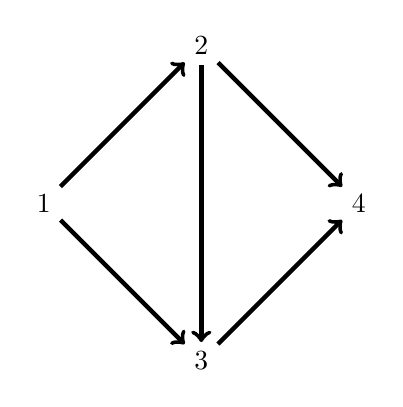
\begin{tikzpicture}[scale=2]
            \node (A) at  (0, 0) {1};
            \node (B) at  (1, 1) {2};
            \node (C) at  (1,-1) {3};
            \node (D) at  (2, 0) {4};
            \draw [ultra thick, ->] (A) -- (B);
            \draw [ultra thick, ->] (A) -- (C);
            \draw<3> [ultra thick, ->] (B) -- (C);
            \draw [ultra thick, ->] (B) -- (D);
            \draw [ultra thick, ->] (C) -- (D);
        \end{tikzpicture}
    \end{minipage}%
\end{frame}

\begin{frame}{First Implemention of {\tt MonadRace}: Sampling}
    \lstinputlisting[firstline=14, lastline=15]
        {code/src/Control/Monad/Race/Sample.hs}
    \begin{itemize}
        \item
            A {\tt Nothing} return-value corresponds to failure.
        \item
            A {\tt Just (a, t)} return-value indicates result {\tt a}
            after time {\tt t}.
    \end{itemize}
\end{frame}

\begin{frame}{First Implemention of {\tt MonadRace}: Sampling --- \tt Monad}
    \lstinputlisting[firstline=17, lastline=30]
        {code/src/Control/Monad/Race/Sample.hs}
\end{frame}

\begin{frame}{First Implemention of {\tt MonadRace}: Sampling --- \tt MonadError}
    \lstinputlisting[firstline=32, lastline=40]
        {code/src/Control/Monad/Race/Sample.hs}
\end{frame}

\begin{frame}{First Implemention of {\tt MonadRace}: Sampling --- \tt MonadProb}
    \lstinputlisting[firstline=42, lastline=45]
        {code/src/Control/Monad/Race/Sample.hs}
\end{frame}

\begin{frame}{First Implemention of {\tt MonadRace}: Sampling --- \tt MonadDelay}
    \lstinputlisting[firstline=47, lastline=48]
        {code/src/Control/Monad/Race/Sample.hs}
\end{frame}

\begin{frame}{First Implemention of {\tt MonadRace}: Sampling --- \tt MonadRace}
    \vspace{-5mm}
    \scalebox{0.9}{%
        \lstinputlisting[firstline=50, lastline=61]
            {code/src/Control/Monad/Race/Sample.hs}
    }
\end{frame}

\begin{frame}{Pros and Cons of Sampling}
    \begin{itemize}
        \item
            Sampling is straight forward and efficient.
        \item
            We could even support more sophisticated delays,
            like ``proper'' uniform delays easily.
        \item
            On the other hand, it would be nice to get \alert{exact} results
            (at least for small examples).
    \end{itemize}
\end{frame}

\begin{frame}{Second Implemention of {\tt MonadRace}: Exact Distribution}
    \lstinputlisting[firstline=26, lastline=27]
        {code/src/Control/Monad/Race/Discrete.hs}
    \begin{itemize}
        \item
            A triple {\tt(t, p, a)} corresponds to result {\tt a}
            being obtained after time {\tt t} with probability {\tt p}.
        \item
            The sum of all {\tt p} in the list, the \alert{weight},
            can be strictly smaller than 1, in which case there is a
            positive probability that the computation \alert{fails}.
        \item
            ``Morally'' we would like
            {\tt Map a (Map t p)}, but again we do not have an
            {\tt Ord}-instance for all {\tt a}.
    \end{itemize}
\end{frame}

\begin{frame}{Second Implemention of {\tt MonadRace}: Exact Distribution --- \tt MonadError}
    \lstinputlisting[firstline=33, lastline=43]
        {code/src/Control/Monad/Race/Discrete.hs}
\end{frame}

\begin{frame}{Second Implemention of {\tt MonadRace}: Exact Distribution --- \tt MonadProb}
    \lstinputlisting[firstline=45, lastline=49]
        {code/src/Control/Monad/Race/Discrete.hs}
\end{frame}

\begin{frame}{Second Implemention of {\tt MonadRace}: Exact Distribution --- \tt MonadDelay}
    \lstinputlisting[firstline=51, lastline=52]
        {code/src/Control/Monad/Race/Discrete.hs}
\end{frame}

\begin{frame}{Second Implemention of {\tt MonadRace}: Exact Distribution --- \tt MonadRace}
    \vspace{-5mm}
    \scalebox{0.9}{%
        \lstinputlisting[firstline=54, lastline=69]
            {code/src/Control/Monad/Race/Discrete.hs}
    }
\end{frame}

\begin{frame}{Example: The ``Diamond''-Network}
    \begin{minipage}{0.7\textwidth}%
        \centering
        \includegraphics<1>[height=0.8\textheight]{images/diamond1.png}
        \includegraphics<2>[height=0.8\textheight]{images/diamond2.png}
    \end{minipage}%
    \begin{minipage}{0.3\textwidth}%
        \centering
        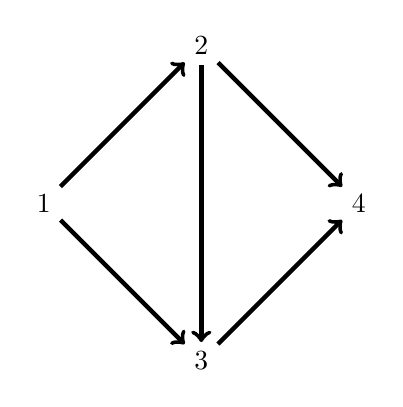
\begin{tikzpicture}[scale=2]
            \node (A) at  (0, 0) {1};
            \node (B) at  (1, 1) {2};
            \node (C) at  (1,-1) {3};
            \node (D) at  (2, 0) {4};
            \draw [ultra thick, ->] (A) -- (B);
            \draw [ultra thick, ->] (A) -- (C);
            \draw<2>[ultra thick, ->] (B) -- (C);
            \draw [ultra thick, ->] (B) -- (D);
            \draw [ultra thick, ->] (C) -- (D);
        \end{tikzpicture}
    \end{minipage}%
\end{frame}

\begin{frame}{Thank you for your attention!}
    \includegraphics[width=2cm]{images/profile.jpg}
    \begin{itemize}
        \item
            EMail: \texttt{lars.bruenjes@iohk.io}
        \item
            Twitter: \texttt{@LarsBrunjes}
        \item
            GitHub: \texttt{https://github.com/brunjlar/}
    \end{itemize}
\end{frame}

\end{document}
